%------------------------------------------------
\section{Introduction}
%------------------------------------------------

\begin{frame}
    \frametitle{Introduction}
    \begin{itemize}
        \item Mainly based on 2 papers:
        \begin{itemize}
            \item Example 7: \textit{Prediction of Pedestrian Dynamics in Complex Architectures with Artificial Neural Networks}
            \item Example 8: \textit{Review of Pedestrian Trajectory Prediction Methods: Comparing Deep Learning and Knowledge-based Approaches}
        \end{itemize}
        \item High level goal:
        \begin{itemize}
            \item \textbf{Implement} neural network and knowledge-based methods
            \item \textbf{Test} and \textbf{compare} on simple scenarios
        \end{itemize}
    \end{itemize}
\end{frame}

\begin{frame}
    \frametitle{Difference between neural and knowledge-based approach}
    \begin{figure}
        \centering
    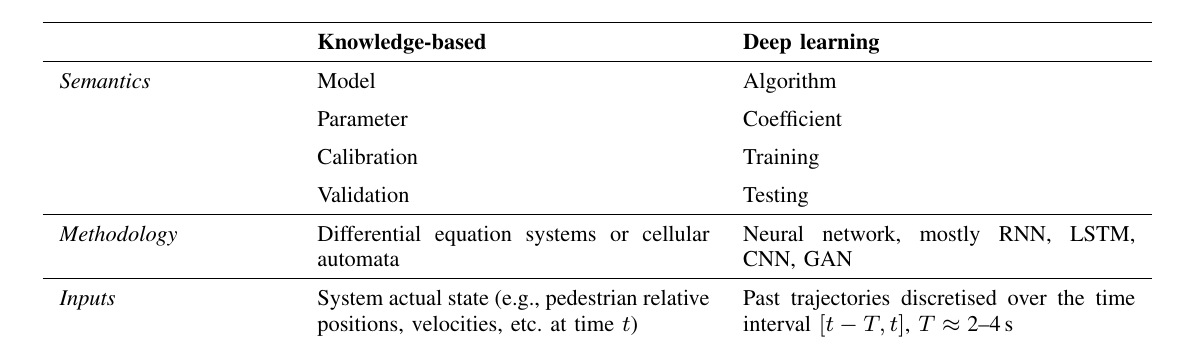
\includegraphics[width=1\textwidth]{Images/cappaper.png}
    \end{figure}
\end{frame}

%------------------------------------------------
\section{Dataset}
%------------------------------------------------

\begin{frame}
    \frametitle{Dataset introduction}
    \begin{itemize}
    \item Dokumentation von Versuchen zur Personenstromdynamik - report for Project Hermes, Bergische Universit{\"a}t Wuppertal
    \item data is structured in a csv table : pedestrian id, time, x, y, z 
    \item we remove the z coordinate as it is constant for each pedestrian
    \item different pedestrians have their speeds measured at different time spans (they are released gradually)
    \item the time is measured in 1/16s the position in cm, origin is chosen arbitrarily
    \end{itemize}

    \begin{figure}
        \centering
        \subfigure[Numpy data dump]{
        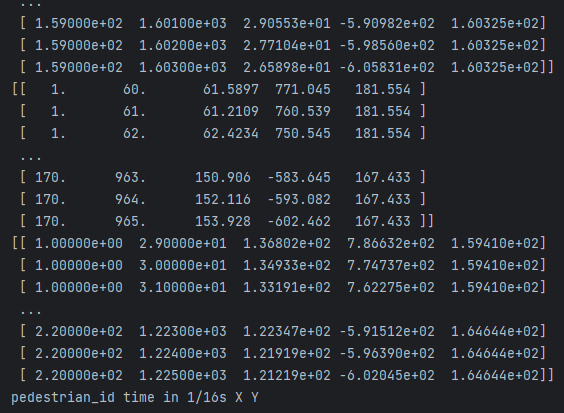
\includegraphics[width=0.2\textwidth]{Images/Screenshot 2024-01-24 130917.png}}
    \end{figure}
\end{frame}

\begin{frame}
    \frametitle{Dataset exploration}
    \begin{itemize}
        \item UO - unidirektional offen 
        \item one directional bottlenecked corridor scenario, the width of the corridor was 1.8 m, the width of the bottleneck was varied 0.7, 0.95 1.2 and 1.8m
    \end{itemize}
    \begin{figure}
        \centering
        \subfigure[experiment diagram]{
        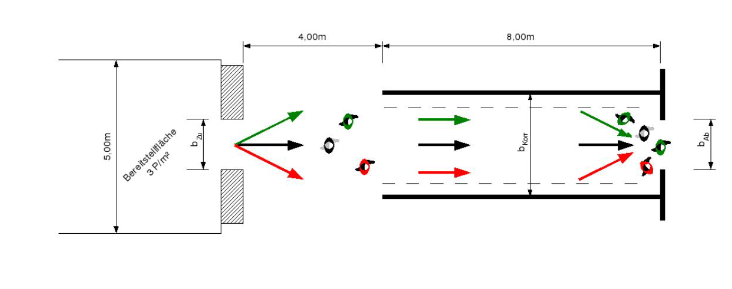
\includegraphics[width=0.3\textwidth]{Images/Screenshot 2024-01-22 133232.png}}
        \subfigure[experiment table]{
        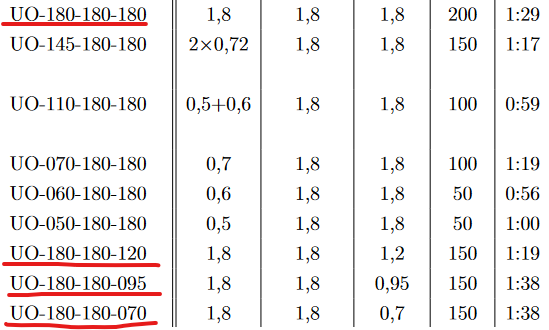
\includegraphics[width=0.3\textwidth]{Images/Screenshot 2024-01-24 150959.png}}
    \end{figure}
\end{frame}

\begin{frame}
    \frametitle{Dataset exploration}
    \begin{itemize}
        \item UG - unidirektional geschlossen 
        \item one directional track oval shaped track scenario
        \item number of pedestrians was varied - 15, 30, 60, 85, 95, 110, 140, 230
        \item track was 1.8m wide, measurement area was 6m long, inner diameter was 2 m
        \item pedestrians took time to start moving was high density (85+ people)
    \end{itemize}
    \begin{figure}
        \centering
        \subfigure[experiment diagram]{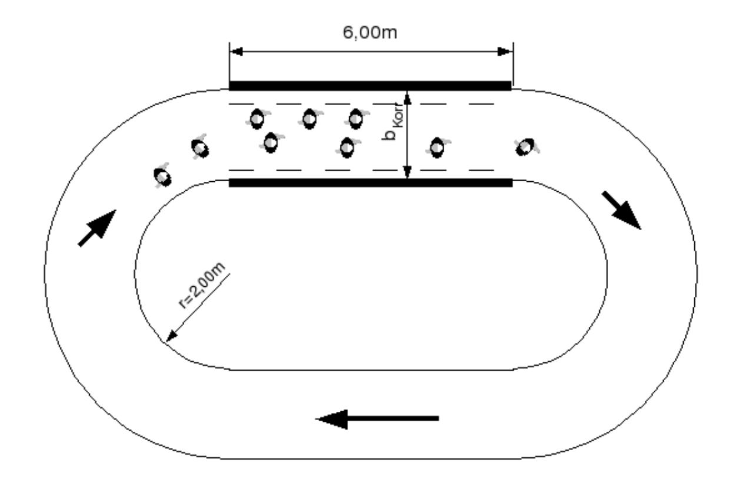
\includegraphics[width=0.3\textwidth]{Images/Screenshot 2024-01-22 133031.png}}
        \subfigure[experiment table]{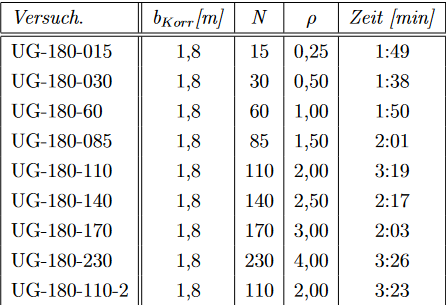
\includegraphics[width=0.3\textwidth]{Images/Screenshot 2024-01-24 150904.png}}
    \end{figure}
\end{frame}

\begin{frame}
    \begin{figure}
        \centering
        \subfigure[no bottleneck]{
        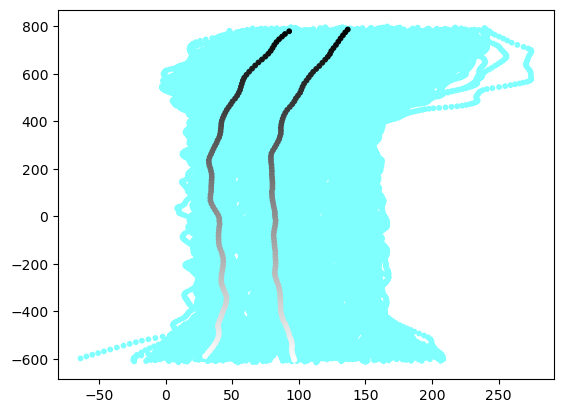
\includegraphics[width=0.4\textwidth]{Images/corridor_no_bottleneck.png}}
        \subfigure[most bottlenecked]{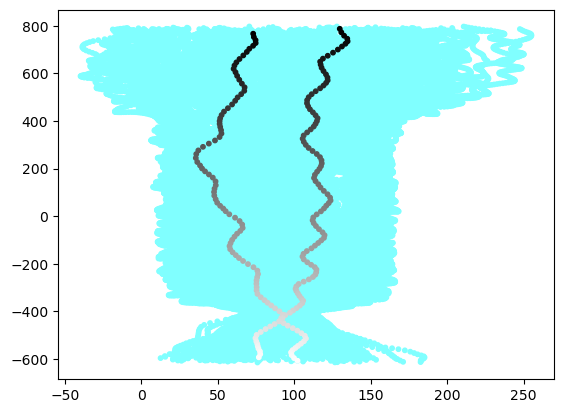
\includegraphics[width=0.4\textwidth]{Images/corridor_most_bottleneck.png}}
        \caption{unidirektional geschlossen pedestrian trajectories (the trajectories of two chosen pedestrians progress black to white)}
    \end{figure}
\end{frame}

\begin{frame}
    \begin{figure}
        \centering
        \subfigure[fewest people]{
        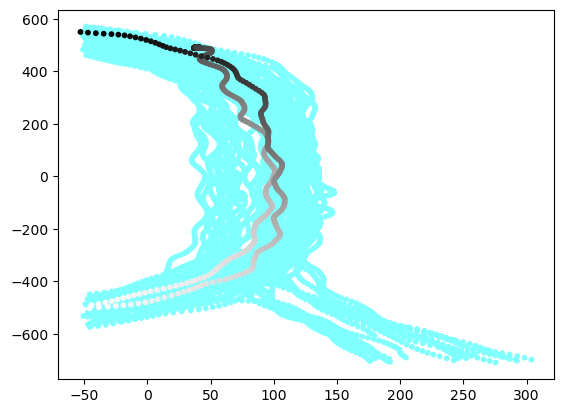
\includegraphics[width=0.4\textwidth]{Images/track_fewest_people.png}}
        \subfigure[most people]{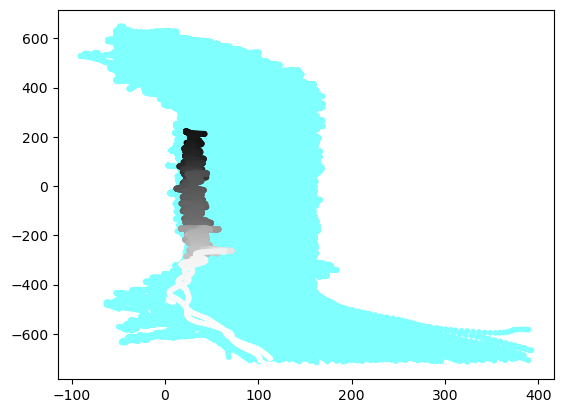
\includegraphics[width=0.4\textwidth]{Images/track_most_people.png}}
        \caption{unidirektional ofnnen pedestrian trajectories (the trajectories of two chosen pedestrians progress black to white)}
    \end{figure}
\end{frame}

%------------------------------------------------
\section{Implementing the models}
%------------------------------------------------

\begin{frame}
    \frametitle{Implementation of knowledge-based model}
    \begin{itemize}
        \item Microscopic speed-based model (Weidmann, 1993)
        \item A non-linear function of mean spacing with three parameters
        \begin{align*}
        W&(\overline{s}_K ,v_0, T, l)=v_0\left( 1-e^{\frac{l-\overline{s}_K}{v_0 T}}\right)\\
        \overline{s}_K &=\frac{1}{K}\sum_{i}\sqrt{(x-x_i)^2+(y-y_i)^2}
        \end{align*}
        \item Where
        \begin{itemize}
            \item $\overline{s}_K$ is mean Euclidean spacing to $K$ closest neighbours
            \item $T$ is following time gap with neighbours
            \item $v_0$ is pedestrian speed in free situation
            \item $l$ physical size of pedestrian in stopped situation
        \end{itemize}
    \end{itemize}
\end{frame}

\begin{frame}
    \frametitle{Implementation of neural network}
    \begin{itemize}
        \item Feed-forward multi-layer perceptron
        \item Fully connected hidden layers $h$ with sigmoid activation function
        \item Input: 
        \begin{itemize}
            \item $x, y$ positions
            \item $v, u$ velocities
            \item $\overline{s}_K$ mean distance spacing
        \end{itemize}
        \item Output: Prediction of pedestrian speed
    \end{itemize}
\end{frame}

\begin{frame}
    \frametitle{Implementation of neural network}
    The four neural networks with different inputs.  
    \begin{itemize}
        \item Relative positions to $K$ closest neighbors.\\
        $NN_1 = NN_1(x_i - x, y_i - y, 1 \leq i \leq K)$
        \item Relative positions and velocities to $K$ closest neighbors. 
        $NN_2 = NN_2(x_i - x, y_i - y,v_i - v,u_i -u, 1 \leq i \leq K)$
        \item Relative positions with mean distance spacing $\bar s_K$\\
        $NN_3 = NN_3(\bar s_K ,(x_i - x, y_i - y, 1 \leq i \leq K))$
        \item Relative positions and velocities with mean distance spacing $\bar s_K$\\
        $NN_4 = NN_4(\bar s_K,(x_i - x, y_i - y,v_i - v,u_i -u, 1 \leq i \leq K))$
    \end{itemize}
\end{frame}

%------------------------------------------------
\section{Discussing the models}
%------------------------------------------------

\begin{frame}
    \frametitle{Comparison between approaches}
    \begin{itemize}
        \item Metrics for testing
        \begin{itemize}
            \item Average Displacement Error (ADE)
            \item Final Displacement Error (FDE)
        \end{itemize}
        \item Testing method
        \begin{itemize}
            \item Use testing set to evaluate
            \item Comparing predictions using metrics
        \end{itemize}
        \item Expected results
        \begin{itemize}
            \item DL outperforms KB
            \item KB outperforms DL (insufficient data)
        \end{itemize} 
    \end{itemize}
\end{frame}

\begin{frame}
    \frametitle{Comparison between approaches}
    \begin{itemize}
    \item Benefits:
        \begin{itemize}
            \item DL: High accuracy, complex interaction learning.
            \item KB: Theoretical clarity, effective in crowds.
        \end{itemize}
    \item Drawbacks:
        \begin{itemize}
            \item DL: Needs large data, lacks interpretability.
            \item KB: Limited to average behavior, less flexible.
        \end{itemize}
    \item Challenges:
        \begin{itemize}
            \item DL: Generalization, model complexity.
            \item KB: Adapting to new scenarios, bias in models.
        \end{itemize}
\end{itemize}
\end{frame}

\begin{frame}
    \frametitle{Conclusion and Future work}
    \begin{itemize}
        \item Both DL and KB have their strengths and limitations
        \item Future work
        \begin{itemize}
            \item Hybrid Approach
            \item DL Expansion
            \item Robustness, Input Variables
        \end{itemize}
    \end{itemize}
\end{frame}


\begin{frame}
    \begin{center}
        \Huge{Thank you for your attention!}
    \end{center}
\end{frame}

%------------------------------------------------
\section{References}
%------------------------------------------------

\begin{frame} % Use [allowframebreaks] to allow automatic splitting across slides if the content is too long
	\frametitle{References}
	\begin{columns}
    \begin{column}{0.5\textwidth}  %%<--- LEFT COLUMN
        \begin{thebibliography}{99} % Beamer does not support BibTeX so references must be inserted manually as below, you may need to use multiple columns and/or reduce the font size further if you have many references
    		\footnotesize % Reduce the font size in the bibliography
            \bibitem[Tordeux et al., 2020]{p1}
               Tordeux et al. (2020)
                \newblock Prediction of pedestrian dynamics in complex architectures with artificial neural networks
                \newblock \emph{Journal of intelligent transportation systems} Vol 24, 556-568. Taylor \& Francis.
        
            \bibitem[Korbmacher et al., 2022]{p2}
               Korbmacher et al. (2022)
                \newblock Review of pedestrian trajectory prediction methods: Comparing deep learning and knowledge-based approaches
                \newblock \emph{IEEE Transactions on Intelligent Transportation Systems} IEEE.
    	\end{thebibliography}
    \end{column}
    \begin{column}{0.5\textwidth}  %%<--- RIGHT COLUMN
        \begin{thebibliography}{99} % Beamer does not support BibTeX so references must be inserted manually as below, you may need to use multiple columns and/or reduce the font size further if you have many references
    		\footnotesize % Reduce the font size in the bibliography
            \bibitem[Weidmann, 1993]{p3}
               Weidmann (1993)
                \newblock Transporttechnik der Fussgaenger -\\
                Transporttechnische Eigenschaften des Fussgarngerverkehrs, Literaturauswertung
                \newblock \emph{IVT Schriftenreihe} Vol 90. ETH Zurich.
    	\end{thebibliography}
    \end{column}
    \end{columns}
\end{frame}

%------------------------------------------------
\section{}
%------------------------------------------------
%----------------------------------------------------------------------------------------
%	CLOSING SLIDE
%----------------------------------------------------------------------------------------

\bgroup
\setbeamercolor{background canvas}{bg=black}
\begin{frame}[plain] % The optional argument 'plain' hides the headline and footline
%----------------------------------------------------------------------------------------
%	BLANK SLIDE
%----------------------------------------------------------------------------------------
\end{frame}
\egroup